% Copyright 2004 by Till Tantau <tantau@users.sourceforge.net>.
%
% In principle, this file can be redistributed and/or modified under
% the terms of the GNU Public License, version 2.
%
% However, this file is supposed to be a template to be modified
% for your own needs. For this reason, if you use this file as a
% template and not specifically distribute it as part of a another
% package/program, I grant the extra permission to freely copy and
% modify this file as you see fit and even to delete this copyright
% notice. 

% \UseRawInputEncoding
\documentclass{beamer}

% There are many different themes available for Beamer. A comprehensive
% list with examples is given here:
% http://deic.uab.es/~iblanes/beamer_gallery/index_by_theme.html
% You can uncomment the themes below if you would like to use a different
% one:
%\usetheme{AnnArbor}
%\usetheme{Antibes}
%\usetheme{Bergen}
%\usetheme{Berkeley}
%\usetheme{Berlin}
%\usetheme{Boadilla}
%\usetheme{boxes}
%\usetheme{CambridgeUS}
%\usetheme{Copenhagen}
%\usetheme{Darmstadt}
%\usetheme{default}
%\usetheme{Frankfurt}
%\usetheme{Goettingen}
%\usetheme{Hannover}
%\usetheme{Ilmenau}
%\usetheme{JuanLesPins}
%\usetheme{Luebeck}
\usetheme{Madrid}
%\usetheme{Malmoe}
%\usetheme{Marburg}
%\usetheme{Montpellier}
%\usetheme{PaloAlto}
%\usetheme{Pittsburgh}
%\usetheme{Rochester}
%\usetheme{Singapore}
%\usetheme{Szeged}
%\usetheme{Warsaw}

\usepackage{pgfgantt}
\usepackage{todonotes}
\usepackage{media9}
\usepackage{fontawesome5}
\usepackage{subfigure}
\usepackage{booktabs,array}
\usepackage{tabulary}
\usepackage{caption}
\usepackage{subfigure}
\usepackage{siunitx}

\usepackage[ruled, vlined, linesnumbered]{algorithm2e} % For algorithms

\usepackage{amsmath} % For typesetting math

% Customize Warsaw color 
\setbeamercolor*{palette primary}{use=structure,fg=white,bg=red!50!black}
\setbeamercolor*{palette secondary}{use=structure,fg=white,bg=red!60!black}
\setbeamercolor*{palette tertiary}{use=structure,fg=white,bg=red!70!black}

% Customize Warsaw block title and background colors
\setbeamercolor{block title}{bg=red!50!black,fg=white}

\setbeamertemplate{bibliography item}{\insertbiblabel}  % insert bibliography numbers instead of symbol
\setbeamertemplate{caption}[numbered] % adds the figure or table number to the caption.



\title[Robotic Cart System (Proposal)]{Robotic Cart System}

% % A subtitle is optional and this may be deleted
\subtitle{Product Proposal}

\author[K.~Allen, D.~Beebe, J.~Braker]{Kallistah~Allen \and Darrah~Beebe \and
Jason~Braker
Advisors:~Dr.~Suruz~Miah \and Dr.~Prasad~Shastry}
% - Give the names in the same order as the appear in the paper.
% - Use the \inst{?} command only if the authors have different
%   affiliation.

\institute[Bradley University] % (optional, but mostly needed)
{
  Department of Electrical and Computer Engineering\\
  Bradley University\\
  1501 W. Bradley Avenue\\
  Peoria, IL, 61625, USA
}
% - Use the \inst command only if there are several affiliations.
% - Keep it simple, no one is interested in your street address.

\date[December~1,~2020]{Tuesday, December~1,~2020}

% - Either use conference name or its abbreviation.
% - Not really informative to the audience, more for people (including
%   yourself) who are reading the slides online

\logo{\hfill\href{http://www.bradley.edu}{
\includegraphics[width=0.75cm]{figs/logoBU1-Print}}}  % place logo in every page 


% \subject{Mobile Robot Localization}
% This is only inserted into the PDF information catalog. Can be left
% out. 

% If you have a file called "university-logo-filename.xxx", where xxx
% is a graphic format that can be processed by latex or pdflatex,
% resp., then you can add a logo as follows:

% \pgfdeclareimage[height=0.5cm]{university-logo}{university-logo-filename}
% \logo{\pgfuseimage{university-logo}}

% Delete this, if you do not want the table of contents to pop up at
% the beginning of each subsection:
\AtBeginSubsection[]
{
  \begin{frame}<beamer>{Outline}
    \tableofcontents[currentsection,currentsubsection]
  \end{frame}
}

% Delete this, if you do not want the table of contents to pop up at
% the beginning of each section:
\AtBeginSection[]
{
  \begin{frame}<beamer>{Outline}
    \tableofcontents[currentsection]
  \end{frame}
}

% Let's get started
\begin{document}

\begin{frame}
  \titlepage
\end{frame}

\begin{frame}{Outline} 
  \tableofcontents%[pausesections]
  % You might wish to add the option [pausesections]
\end{frame}

% Section and subsections will appear in the presentation overview
% and table of contents.
\section{Introduction}

\begin{frame}{Introduction}
  \begin{center}
    \href{videos/proposalVideo.mp4}{
\includegraphics[width=0.8\textwidth]{figs/img/proposalVideoTitle}}
  \end{center}
  % \begin{center}
  %   \includemedia[
  %     width=\textwidth,
  %     height=0.7\textheight,
  %     label=proposalVideo,
  %     % activate=onclick,
  %     % playbutton=fancy,
  %     addresource=videos/proposalVideo.mp4,
  %     flashvars={source=videos/proposalVideo.mp4}]
  %     {}{VPlayer.swf}
  %     \\
  %     % \mediabutton[
  %     %   mediacommand=proposalVideo:playPause,
  %     %   overface=\color{blue}{\fbox{\strut \faPause\ \faPlay}},
  %     %   downface=\color{red}{\fbox{\strut \faPause\ \faPlay}}
  %     % ]{}
  %     % \mediabutton[
  %     %   mediacommand=proposalVideo:setSource
  %     %   [(videos/proposalVideo.mp4)]]{\fbox{Introduction Video}}
  % \end{center}
\end{frame}

\begin{frame}{Problem Statement}
  \begin{block}{Problem Statement}
    \begin{LARGE}
      Design a robotic cart that follows the user.
    \end{LARGE}
  \end{block}
  \pause
  \begin{block}{Proposed Solution}
    \begin{LARGE}
      Utilize analog wireless signal strength to locate and then follow the user.
    \end{LARGE}
  \end{block}
\end{frame}

\begin{frame}{Introduction}{}
  % applications of mobile robot navigation and problem description
  \begin{block}{Applications of Mobile Carts}
    \begin{itemize}
      \item Mail delivery
      \item Transferring files in offices
      \item Carrying medical supplies in Hospitals (Fig.\ref{fig:medCart})
      \item Carrying materials and tools in factories (Fig. \ref{fig:factCart})
      \item Shopping carts for ease of use and people with disabilities
    \end{itemize}
  \end{block}
      \begin{figure}
      \centering
      \begin{minipage}[t]{0.5\textwidth}
        \centering
        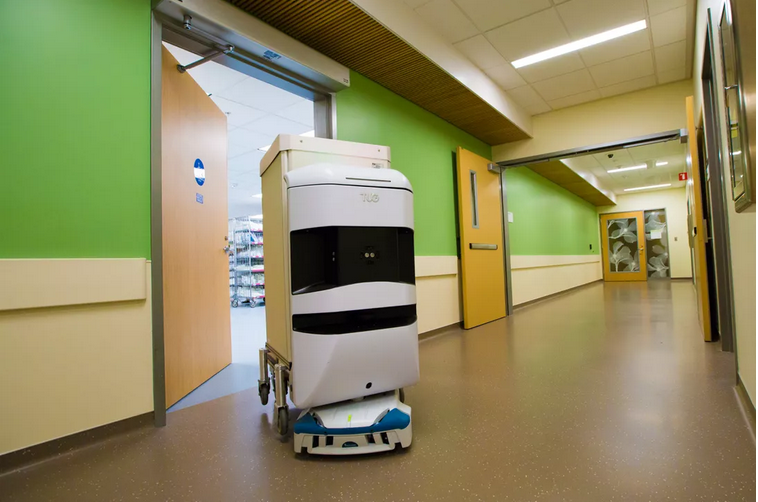
\includegraphics[height=3cm]{figs/img/MedicalRoboticCart}
        \caption{Medical Mobile Robotic Cart}
        \label{fig:medCart}
      \end{minipage}
      \begin{minipage}[t]{0.4\textwidth}
        \centering
        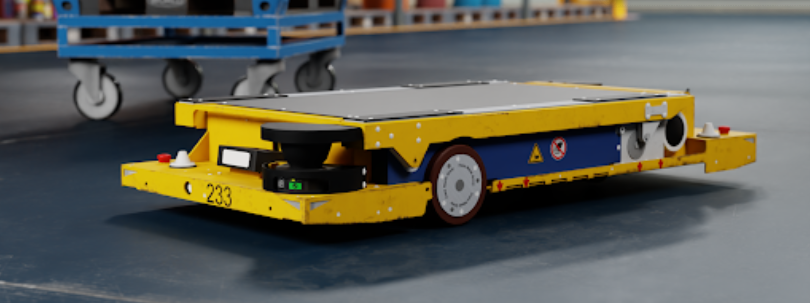
\includegraphics[height=2.0cm]{figs/img/FactoryRoboticCart}
        \caption{Factory Mobile Robotic Cart}
        \label{fig:factCart}
      \end{minipage}
    \end{figure}
\end{frame}

%----------------------------------

\section{Literature Review}

\begin{frame}{Literature Review}
  \begin{block}{Existing Solution}
        Mobile platform interface with ultrasound and radio transmission technology~\cite{Sales2016-CompaRob}
  \end{block}
    \begin{figure}[b]
        \centering
        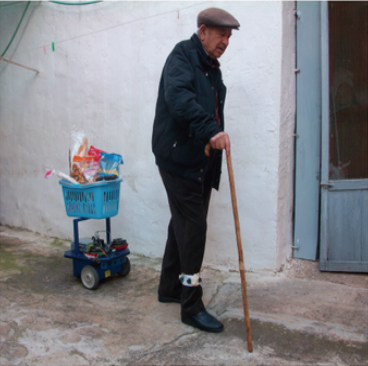
\includegraphics[width=0.45\textwidth]{figs/img/CompaRob}
        \caption{CompaRob}
        %\label{fig:sysBlockDiag}
    \end{figure}
\end{frame}

%----------------------------------

\begin{frame}{Literature Review}
  \begin{block}{Existing Solution}
        Gated Recurrent Unit (GRU) network with LiDAR sensor and camera to map the customer~\cite{islam_lam_fukuda_kobayashi_kuno_2019}
  \end{block}
    \begin{figure}[b]
        \centering
        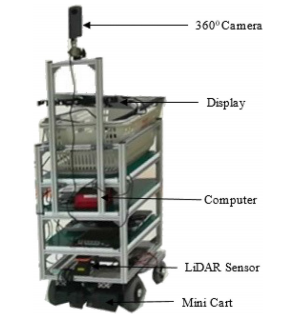
\includegraphics[width=0.40\textwidth]{figs/img/ShoppingSuportRobot}
        \caption{Shopping Support Robot}
        %\label{fig:sysBlockDiag}
    \end{figure}
\end{frame}

%----------------------------------

\begin{frame}{Literature Review}
  \begin{block}{Existing Solution}
    Arduino MEGA 2560, six ultrasonic sensors, two DC motors with Pulse Width Modulation (PWM), an Android Studio IDE device, and Bluetooth~\cite{Rawashdeh2017-Person}
  \end{block}
    \begin{figure}[b]
        \centering
        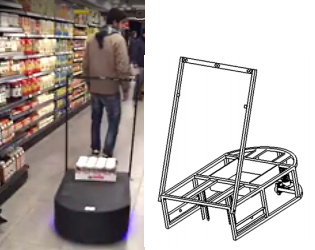
\includegraphics[width=0.50\textwidth]{figs/img/SmartCart}
        \caption{Smart Cart Robot}
        %\label{fig:sysBlockDiag}
    \end{figure}
\end{frame}

%----------------------------------

\begin{frame}{Existing Solutions}
  \begin{block}{Problems}
    \begin{itemize}
      \item Require line-of-sight between robot and user
      \item Some require costly dedicated image processing hardware
    \end{itemize}
  \end{block}
  \pause
  \begin{block}{Benefits of Proposed Solution}
    \begin{itemize}
      \item Line-of-sight is not required since analog RF signals will be used
      \item RF components are cost-effective
    \end{itemize}
  \end{block}
\end{frame}

%----------------------------------

% \begin{frame}{Literature Review}
%   \begin{block}{Multipath Interference}
%     \begin{itemize}
%       \item Proposed solutions to multipath interference
%       \begin{itemize}
%         \item Course estimation calculations such as recieved signal strength indicator (RSSI) and time difference of arrival (TDoA)
%         \item IEEE 802.11b wireless Ethernet device to measure RF signals
%         \item Sampling radio signal strength (RSS) at discrete points without too much deviation from the robot's desired position
%       \end{itemize}
%     \end{itemize}
%   \end{block}
%       \begin{figure}[b]
%         \centering
%         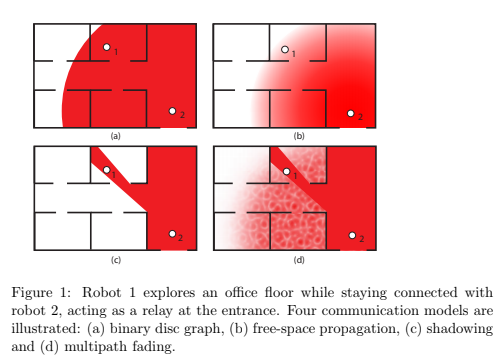
\includegraphics[width=0.40\textwidth]{figs/img/MultipathFading}
%         \caption{Multipath Fading}
%         %\label{fig:sysBlockDiag}
%     \end{figure}
% \end{frame}

% %----------------------------------

% \begin{frame}{Literature Review}
%   \begin{block}{Challenges}
%     \begin{itemize}
%       \item Communication between the robot and the remote
%       \item Buffer distance between the robotic cart and the customer without using line of sight sensing
%     \end{itemize}
%   \end{block}
% \end{frame}

%----------------------------------

\section{System Requirements}
\begin{frame}{System Requirements}
  \begin{block}{Specifications}
    \begin{itemize}
      \item Cart should be able to follow the remote target
      \item Cart should maintain a distance of 1 to 1.5 meters from the remote target.
      \item Cart should be able to travel at minimum 1 m/s
      \item Cart should not require line-of-sight to follow remote
     \end{itemize}
  \end{block}
\end{frame}

%----------------------------------

\section{System Architecture}
\subsection{Block Diagrams}
\begin{frame}{Block Diagrams}
  \begin{block}{}
    Two main components of system
    \begin{itemize}
      \item Mobile Cart
      \item Remote Target
    \end{itemize}
    System Block Diagram shown in Figure \autoref{fig:sysBlockDiag}
  \end{block}
  \begin{figure}[b]
    \centering
    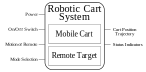
\includegraphics[width=0.75\textwidth]{figs/system_block_diagram_2}
    \caption{Block Diagram of the Robotic Cart System}
    \label{fig:sysBlockDiag}
  \end{figure}
\end{frame}

\begin{frame}{Block Diagrams}
  \begin{block}{}
    Remote Target Subsystem Block Diagram shown in Figure \autoref{fig:sysRemoteBlockDiag}
  \end{block}
  \begin{figure}[b]
    \centering
    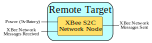
\includegraphics[width=\textwidth]{figs/remote_target_block_diagram}
    \caption{Block Diagram of Remote Target Subsystem}
    \label{fig:sysRemoteBlockDiag}
  \end{figure}
\end{frame}

\begin{frame}{Block Diagrams}
  \begin{block}{}
    Mobile Cart Subsystem Block Diagram shown in Figure \autoref{fig:sysMobileBlockDiag}
  \end{block}
  \begin{figure}[b]
    \centering
    \includegraphics[width=0.9\textwidth]{figs/mobile_cart_block_diagram}
    \caption{Block Diagram of Mobile Cart Subsystem}
    \label{fig:sysMobileBlockDiag}
  \end{figure}
\end{frame}

%----------------------------------

\subsection{System Components}

\begin{frame}{System Components}
  \begin{block}{Main Components}
    \begin{itemize}
      \item Budget Bot mobile robot chassis (Fig. \ref{fig:budgetBotChassis})
      \item BeagleBone Blue (Fig. \ref{fig:beagleboneBlue})
      \item XBee S2C module (Fig. \ref{fig:XBeeModule})
    \end{itemize}
  \end{block}
  \begin{figure}
    \centering
    \begin{minipage}[t]{0.32\textwidth}
      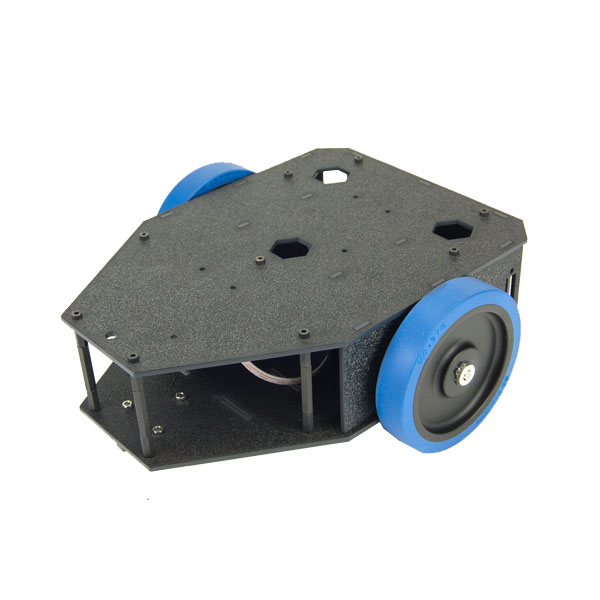
\includegraphics[width=1\textwidth]{figs/img/budgetbot_chassis}
      \caption{Budget Bot Chassis}
      \label{fig:budgetBotChassis}
    \end{minipage}%
    \begin{minipage}[t]{0.32\textwidth}
      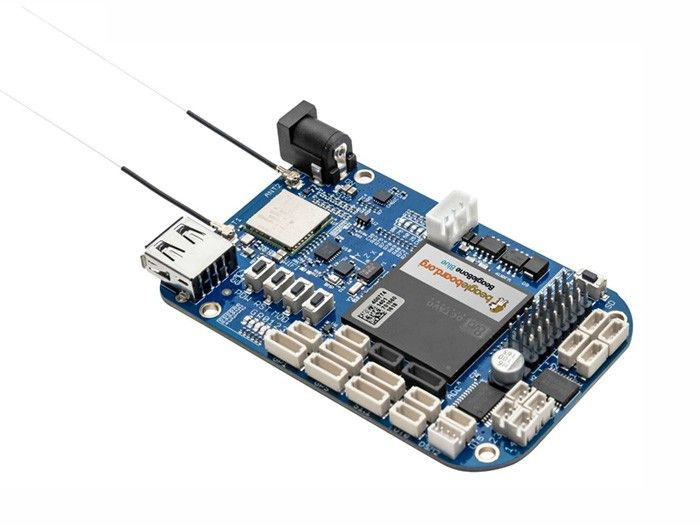
\includegraphics[width=1\textwidth]{figs/img/beaglebone_blue}
      \caption{BeagleBone Blue}
      \label{fig:beagleboneBlue}
    \end{minipage}
    \begin{minipage}[t]{0.32\textwidth}
      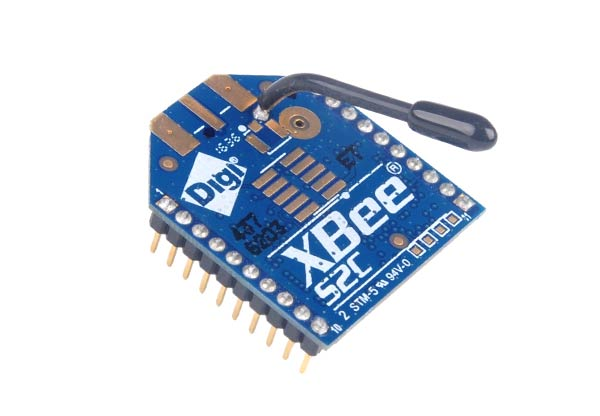
\includegraphics[width=1\textwidth]{figs/img/Xbee-S2C-Module}
      \caption{XBee S2C Module}
      \label{fig:XBeeModule}
    \end{minipage}
  \end{figure}
\end{frame}

%----------------------------------

\begin{frame}{System Components}
    \begin{block}{Reflector Array}
    Two designs for reflector array:
    \begin{itemize}
      \item Paraboloidal Reflector (Fig. \ref{fig:parabolodialReflector})
      \item Combined Parabolic/Paraboloidal Reflector (Fig. \ref{fig:parabolicReflector})
    \end{itemize}
    \end{block}
    \begin{figure}
      \centering
      \begin{minipage}[t]{0.5\textwidth}
        \centering
        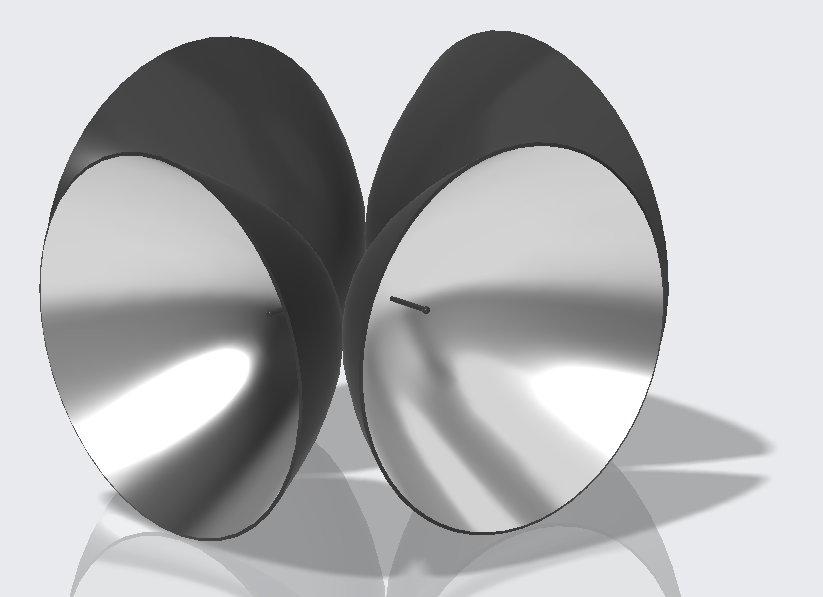
\includegraphics[height=3.5cm]{figs/img/paraboloidalReflector}
        \caption{Paraboloidal Reflector Model}
        \label{fig:parabolodialReflector}
      \end{minipage}
      \begin{minipage}[t]{0.4\textwidth}
        \centering
        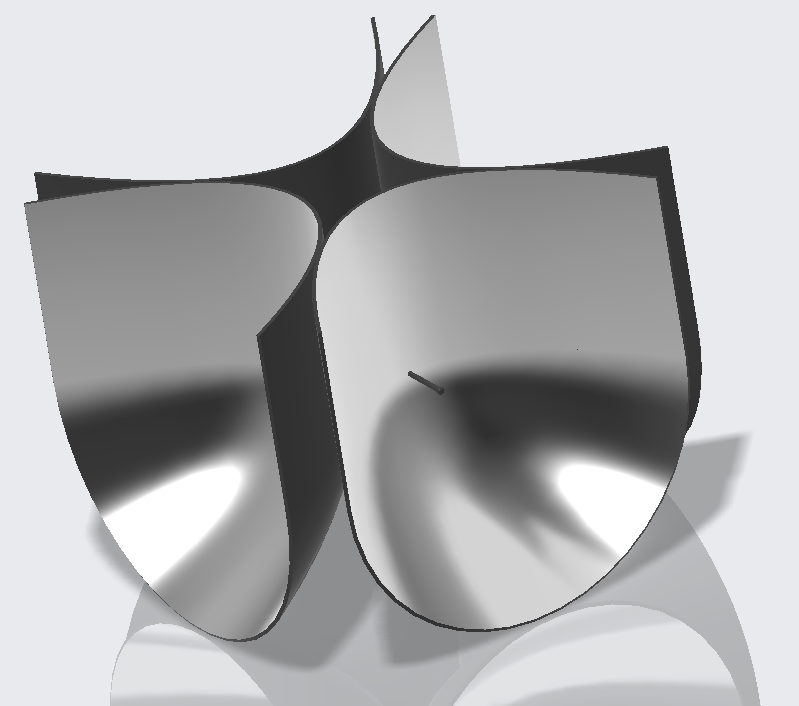
\includegraphics[height=3.5cm]{figs/img/parabolicReflector}
        \caption{Combined Parabolic/Paraboloidal Reflector}
        \label{fig:parabolicReflector}
      \end{minipage}
    \end{figure}
\end{frame}

\begin{frame}{System Components}
  \begin{table}[h!]
      \centering
      \begin{tabular}{c|c}
          \toprule
          \textbf{Quantity} & \textbf{Parts}\\
          \toprule
          2 & Budget Bot Chassis\\
          4 & 10 uF Ceramic Capacitor\\
          4 & LM1117 Regulator\\
          2 & Battery Packs for Budget Bot\\
          8 & 9V Batteries\\
          4 & Solderable PCB Boards\\
          3 & XBee USB Adapter\\
          \bottomrule
          %\multicolumn{2}{r|}{\textbf{Total}} & \$ 562.34\\
          %\bottomrule
      \end{tabular}
      \caption{Parts Available in Laboratory}
      \label{tab:Partslablist}
  \end{table}
\end{frame}

\begin{frame}{System Components}
  \begin{table}[h!]
    \centering
    \begin{tabular}{c|c|c}
      \toprule
      \textbf{Quantity} & \textbf{Parts} & \textbf{Price}\\
      \toprule
      4 & Pololu 37D Metal Gaermotor 4751 & \$ 39.95\\
      12 & XBee S2C Module & \$ 23.10\\
      10 & XBee Adapter Board & \$ 4.99\\
      2 & Twotrees 4 Lead Nema 17 Stepper Motor & \$ 9.99\\
      1 & 4-Pin JST SH Connector - 20 Pack & \$ 7.99\\
      1 & 6-Pin JST SH Connector - 10 Pack & \$ 9.99\\
      1 & Aluminum Foil Tape - 2 in x 5 yd & \$ 6.05\\
      \bottomrule
      \multicolumn{2}{r|}{\textbf{Total}} & \$ 562.34\\
      \bottomrule
    \end{tabular}
    \caption{Purchased parts for the Robotic Cart Project}
    \label{tab:Partslist}
  \end{table}
\end{frame}



%----------------------------------

\subsection{Operation of Mobile Cart System}
\begin{frame}{Operation of Mobile Cart System}
  \begin{figure}
    \centering
    \begingroup
    \tiny
    % Graphic for TeX using PGF
% Title: S:\Senior Project\seniorProject2-2020-21-Docs\figs\dia\systemOperationFlowchart.dia
% Creator: Dia v0.97.2
% CreationDate: Wed Nov 25 16:20:30 2020
% For: Jason Braker
% \usepackage{tikz}
% The following commands are not supported in PSTricks at present
% We define them conditionally, so when they are implemented,
% this pgf file will use them.
\ifx\du\undefined
  \newlength{\du}
\fi
\setlength{\du}{15\unitlength}
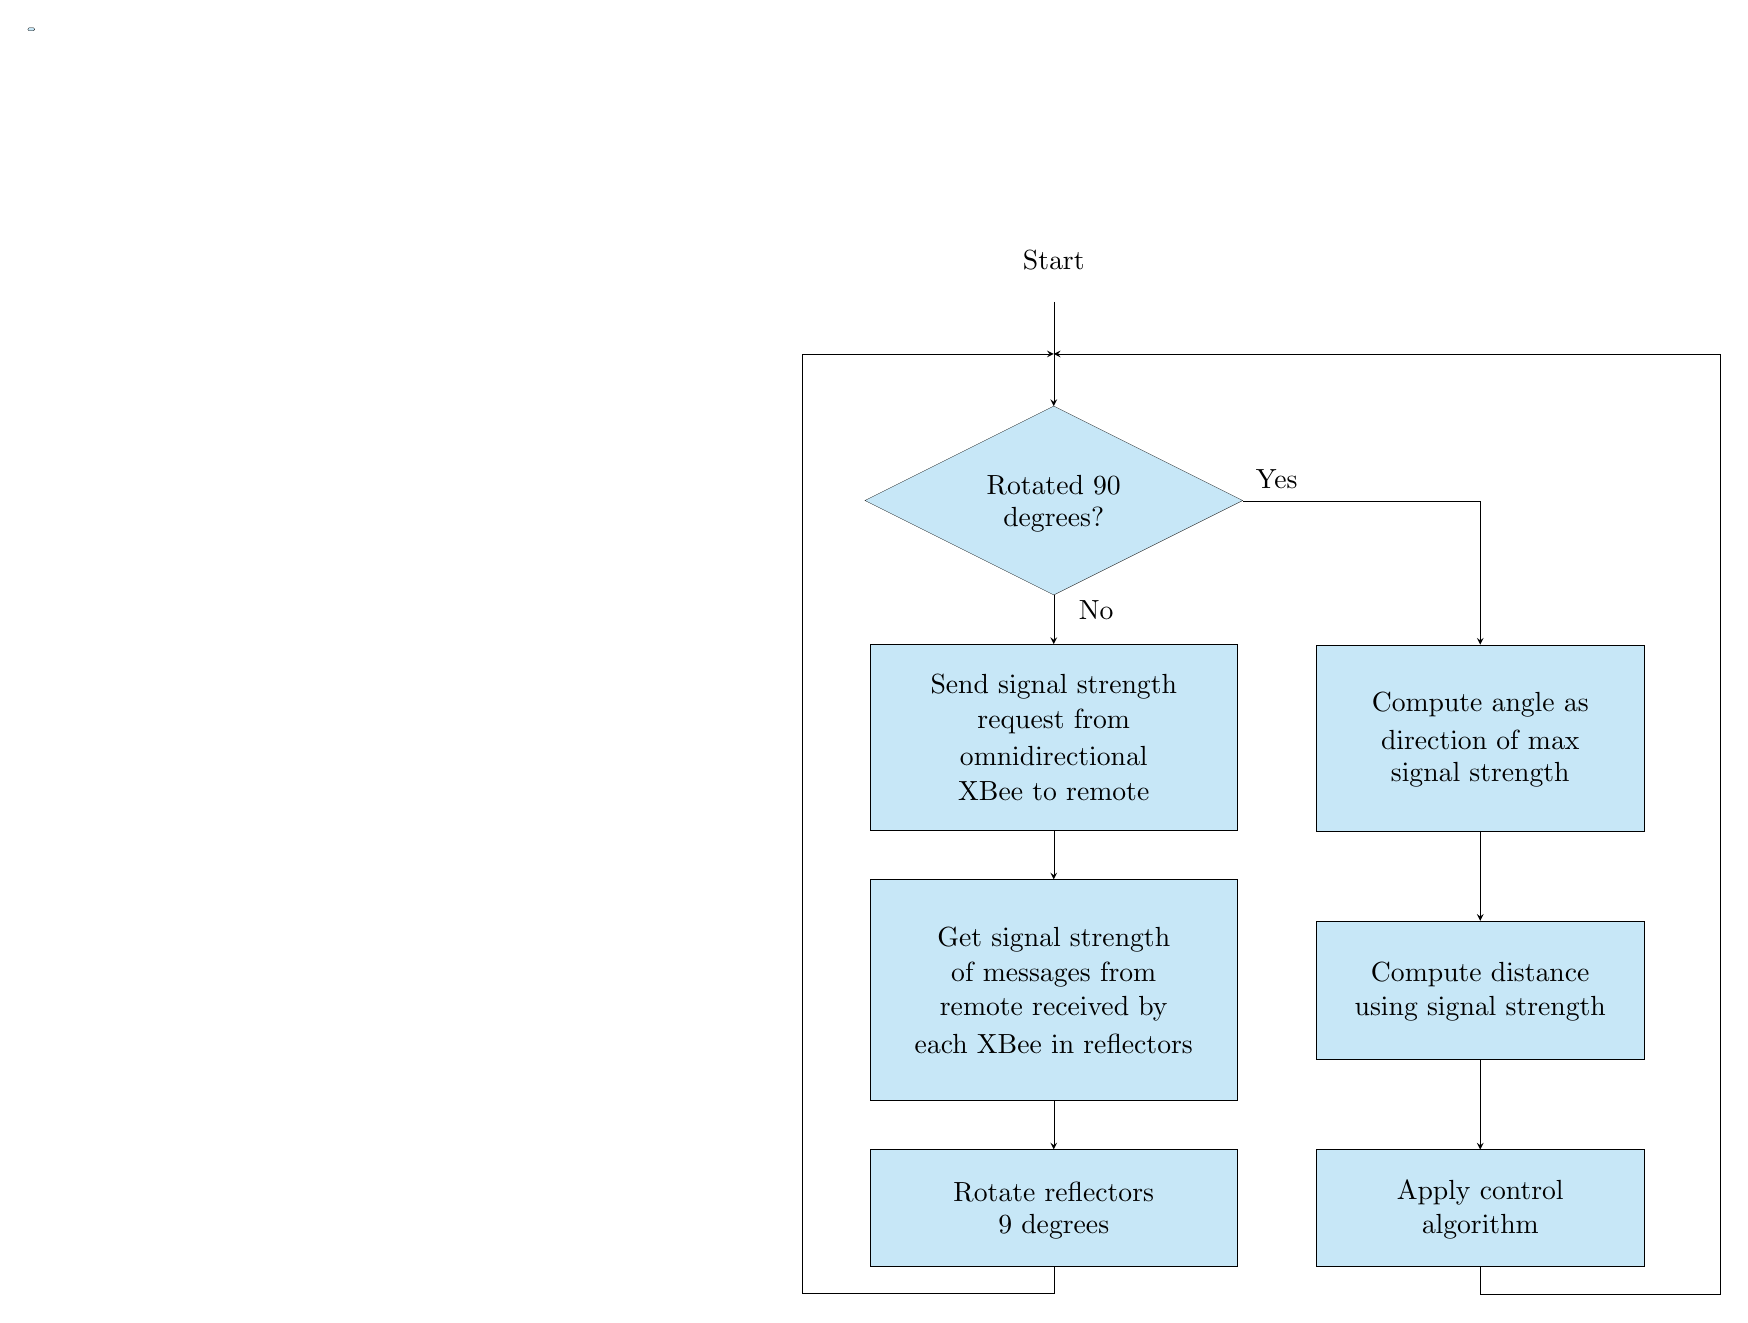
\begin{tikzpicture}[scale=0.55]
\pgftransformxscale{1.000000}
\pgftransformyscale{-1.000000}
\definecolor{dialinecolor}{rgb}{0.000000, 0.000000, 0.000000}
\pgfsetstrokecolor{dialinecolor}
\definecolor{dialinecolor}{rgb}{1.000000, 1.000000, 1.000000}
\pgfsetfillcolor{dialinecolor}
\pgfsetlinewidth{0.100000\du}
\pgfsetdash{}{0pt}
\pgfsetdash{}{0pt}
\pgfsetbuttcap
\pgfsetmiterjoin
\pgfsetlinewidth{0.100000\du}
\pgfsetbuttcap
\pgfsetmiterjoin
\pgfsetdash{}{0pt}
\definecolor{dialinecolor}{rgb}{0.780392, 0.905882, 0.968627}
\pgfsetfillcolor{dialinecolor}
\pgfpathmoveto{\pgfpoint{22.956946\du}{4.485162\du}}
\pgfpathlineto{\pgfpoint{25.983196\du}{4.485162\du}}
\pgfpathcurveto{\pgfpoint{26.401035\du}{4.485162\du}}{\pgfpoint{26.739759\du}{4.932877\du}}{\pgfpoint{26.739759\du}{5.485162\du}}
\pgfpathcurveto{\pgfpoint{26.739759\du}{6.037447\du}}{\pgfpoint{26.401035\du}{6.485162\du}}{\pgfpoint{25.983196\du}{6.485162\du}}
\pgfpathlineto{\pgfpoint{22.956946\du}{6.485162\du}}
\pgfpathcurveto{\pgfpoint{22.539108\du}{6.485162\du}}{\pgfpoint{22.200384\du}{6.037447\du}}{\pgfpoint{22.200384\du}{5.485162\du}}
\pgfpathcurveto{\pgfpoint{22.200384\du}{4.932877\du}}{\pgfpoint{22.539108\du}{4.485162\du}}{\pgfpoint{22.956946\du}{4.485162\du}}
\pgfusepath{fill}
\definecolor{dialinecolor}{rgb}{0.000000, 0.000000, 0.000000}
\pgfsetstrokecolor{dialinecolor}
\pgfpathmoveto{\pgfpoint{22.956946\du}{4.485162\du}}
\pgfpathlineto{\pgfpoint{25.983196\du}{4.485162\du}}
\pgfpathcurveto{\pgfpoint{26.401035\du}{4.485162\du}}{\pgfpoint{26.739759\du}{4.932877\du}}{\pgfpoint{26.739759\du}{5.485162\du}}
\pgfpathcurveto{\pgfpoint{26.739759\du}{6.037447\du}}{\pgfpoint{26.401035\du}{6.485162\du}}{\pgfpoint{25.983196\du}{6.485162\du}}
\pgfpathlineto{\pgfpoint{22.956946\du}{6.485162\du}}
\pgfpathcurveto{\pgfpoint{22.539108\du}{6.485162\du}}{\pgfpoint{22.200384\du}{6.037447\du}}{\pgfpoint{22.200384\du}{5.485162\du}}
\pgfpathcurveto{\pgfpoint{22.200384\du}{4.932877\du}}{\pgfpoint{22.539108\du}{4.485162\du}}{\pgfpoint{22.956946\du}{4.485162\du}}
\pgfusepath{stroke}
% setfont left to latex
\definecolor{dialinecolor}{rgb}{0.000000, 0.000000, 0.000000}
\pgfsetstrokecolor{dialinecolor}
\node at (24.470071\du,5.525162\du){Start};
\pgfsetlinewidth{0.100000\du}
\pgfsetdash{}{0pt}
\pgfsetdash{}{0pt}
\pgfsetbuttcap
{
\definecolor{dialinecolor}{rgb}{0.000000, 0.000000, 0.000000}
\pgfsetfillcolor{dialinecolor}
% was here!!!
\pgfsetarrowsend{stealth}
\definecolor{dialinecolor}{rgb}{0.000000, 0.000000, 0.000000}
\pgfsetstrokecolor{dialinecolor}
\draw (24.470071\du,13.253697\du)--(24.470071\du,14.388015\du);
}
\pgfsetlinewidth{0.100000\du}
\pgfsetdash{}{0pt}
\pgfsetdash{}{0pt}
\pgfsetbuttcap
{
\definecolor{dialinecolor}{rgb}{0.000000, 0.000000, 0.000000}
\pgfsetfillcolor{dialinecolor}
% was here!!!
\pgfsetarrowsend{stealth}
\definecolor{dialinecolor}{rgb}{0.000000, 0.000000, 0.000000}
\pgfsetstrokecolor{dialinecolor}
\draw (24.470071\du,6.485162\du)--(24.470071\du,8.891787\du);
}
\pgfsetlinewidth{0.100000\du}
\pgfsetdash{}{0pt}
\pgfsetdash{}{0pt}
\pgfsetmiterjoin
\pgfsetbuttcap
{
\definecolor{dialinecolor}{rgb}{0.000000, 0.000000, 0.000000}
\pgfsetfillcolor{dialinecolor}
% was here!!!
\pgfsetarrowsend{stealth}
{\pgfsetcornersarced{\pgfpoint{0.000000\du}{0.000000\du}}\definecolor{dialinecolor}{rgb}{0.000000, 0.000000, 0.000000}
\pgfsetstrokecolor{dialinecolor}
\draw (24.470071\du,28.756650\du)--(24.470071\du,29.380791\du)--(18.662017\du,29.380791\du)--(18.662017\du,7.688475\du)--(24.470071\du,7.688475\du);
}}
\pgfsetlinewidth{0.100000\du}
\pgfsetdash{}{0pt}
\pgfsetdash{}{0pt}
\pgfsetmiterjoin
\pgfsetbuttcap
{
\definecolor{dialinecolor}{rgb}{0.000000, 0.000000, 0.000000}
\pgfsetfillcolor{dialinecolor}
% was here!!!
\pgfsetarrowsend{stealth}
{\pgfsetcornersarced{\pgfpoint{0.000000\du}{0.000000\du}}\definecolor{dialinecolor}{rgb}{0.000000, 0.000000, 0.000000}
\pgfsetstrokecolor{dialinecolor}
\draw (28.831982\du,11.072742\du)--(28.831982\du,11.079441\du)--(34.317833\du,11.079441\du)--(34.317833\du,14.401811\du);
}}
% setfont left to latex
\definecolor{dialinecolor}{rgb}{0.000000, 0.000000, 0.000000}
\pgfsetstrokecolor{dialinecolor}
\node[anchor=west] at (28.920363\du,10.565993\du){Yes};
% setfont left to latex
\definecolor{dialinecolor}{rgb}{0.000000, 0.000000, 0.000000}
\pgfsetstrokecolor{dialinecolor}
\node[anchor=west] at (24.833774\du,13.604637\du){No};
\definecolor{dialinecolor}{rgb}{0.780392, 0.905882, 0.968627}
\pgfsetfillcolor{dialinecolor}
\fill (20.230538\du,19.822333\du)--(20.230538\du,24.922333\du)--(28.709605\du,24.922333\du)--(28.709605\du,19.822333\du)--cycle;
\pgfsetlinewidth{0.100000\du}
\pgfsetdash{}{0pt}
\pgfsetdash{}{0pt}
\pgfsetmiterjoin
\definecolor{dialinecolor}{rgb}{0.000000, 0.000000, 0.000000}
\pgfsetstrokecolor{dialinecolor}
\draw (20.230538\du,19.822333\du)--(20.230538\du,24.922333\du)--(28.709605\du,24.922333\du)--(28.709605\du,19.822333\du)--cycle;
% setfont left to latex
\definecolor{dialinecolor}{rgb}{0.000000, 0.000000, 0.000000}
\pgfsetstrokecolor{dialinecolor}
\node at (24.470071\du,21.212333\du){Get signal strength};
% setfont left to latex
\definecolor{dialinecolor}{rgb}{0.000000, 0.000000, 0.000000}
\pgfsetstrokecolor{dialinecolor}
\node at (24.470071\du,22.012333\du){of messages from};
% setfont left to latex
\definecolor{dialinecolor}{rgb}{0.000000, 0.000000, 0.000000}
\pgfsetstrokecolor{dialinecolor}
\node at (24.470071\du,22.812333\du){remote received by};
% setfont left to latex
\definecolor{dialinecolor}{rgb}{0.000000, 0.000000, 0.000000}
\pgfsetstrokecolor{dialinecolor}
\node at (24.470071\du,23.612333\du){each XBee in reflectors};
\definecolor{dialinecolor}{rgb}{0.780392, 0.905882, 0.968627}
\pgfsetfillcolor{dialinecolor}
\fill (24.470071\du,8.891787\du)--(28.831982\du,11.072742\du)--(24.470071\du,13.253697\du)--(20.108161\du,11.072742\du)--cycle;
\pgfsetlinewidth{0.100000\du}
\pgfsetdash{}{0pt}
\pgfsetdash{}{0pt}
\pgfsetmiterjoin
\definecolor{dialinecolor}{rgb}{0.000000, 0.000000, 0.000000}
\pgfsetstrokecolor{dialinecolor}
\draw (24.470071\du,8.891787\du)--(28.831982\du,11.072742\du)--(24.470071\du,13.253697\du)--(20.108161\du,11.072742\du)--cycle;
% setfont left to latex
\definecolor{dialinecolor}{rgb}{0.000000, 0.000000, 0.000000}
\pgfsetstrokecolor{dialinecolor}
\node at (24.470071\du,10.712742\du){Rotated 90};
% setfont left to latex
\definecolor{dialinecolor}{rgb}{0.000000, 0.000000, 0.000000}
\pgfsetstrokecolor{dialinecolor}
\node at (24.470071\du,11.512742\du){degrees?};
\definecolor{dialinecolor}{rgb}{0.780392, 0.905882, 0.968627}
\pgfsetfillcolor{dialinecolor}
\fill (30.525333\du,14.401811\du)--(30.525333\du,18.701811\du)--(38.110333\du,18.701811\du)--(38.110333\du,14.401811\du)--cycle;
\pgfsetlinewidth{0.100000\du}
\pgfsetdash{}{0pt}
\pgfsetdash{}{0pt}
\pgfsetmiterjoin
\definecolor{dialinecolor}{rgb}{0.000000, 0.000000, 0.000000}
\pgfsetstrokecolor{dialinecolor}
\draw (30.525333\du,14.401811\du)--(30.525333\du,18.701811\du)--(38.110333\du,18.701811\du)--(38.110333\du,14.401811\du)--cycle;
% setfont left to latex
\definecolor{dialinecolor}{rgb}{0.000000, 0.000000, 0.000000}
\pgfsetstrokecolor{dialinecolor}
\node at (34.317833\du,15.791811\du){Compute angle as};
% setfont left to latex
\definecolor{dialinecolor}{rgb}{0.000000, 0.000000, 0.000000}
\pgfsetstrokecolor{dialinecolor}
\node at (34.317833\du,16.591811\du){direction of max};
% setfont left to latex
\definecolor{dialinecolor}{rgb}{0.000000, 0.000000, 0.000000}
\pgfsetstrokecolor{dialinecolor}
\node at (34.317833\du,17.391811\du){signal strength};
\definecolor{dialinecolor}{rgb}{0.780392, 0.905882, 0.968627}
\pgfsetfillcolor{dialinecolor}
\fill (30.525333\du,20.777419\du)--(30.525333\du,23.968519\du)--(38.110333\du,23.968519\du)--(38.110333\du,20.777419\du)--cycle;
\pgfsetlinewidth{0.100000\du}
\pgfsetdash{}{0pt}
\pgfsetdash{}{0pt}
\pgfsetmiterjoin
\definecolor{dialinecolor}{rgb}{0.000000, 0.000000, 0.000000}
\pgfsetstrokecolor{dialinecolor}
\draw (30.525333\du,20.777419\du)--(30.525333\du,23.968519\du)--(38.110333\du,23.968519\du)--(38.110333\du,20.777419\du)--cycle;
% setfont left to latex
\definecolor{dialinecolor}{rgb}{0.000000, 0.000000, 0.000000}
\pgfsetstrokecolor{dialinecolor}
\node at (34.317833\du,22.012969\du){Compute distance};
% setfont left to latex
\definecolor{dialinecolor}{rgb}{0.000000, 0.000000, 0.000000}
\pgfsetstrokecolor{dialinecolor}
\node at (34.317833\du,22.812969\du){using signal strength};
\definecolor{dialinecolor}{rgb}{0.780392, 0.905882, 0.968627}
\pgfsetfillcolor{dialinecolor}
\fill (30.525333\du,26.058941\du)--(30.525333\du,28.758941\du)--(38.110333\du,28.758941\du)--(38.110333\du,26.058941\du)--cycle;
\pgfsetlinewidth{0.100000\du}
\pgfsetdash{}{0pt}
\pgfsetdash{}{0pt}
\pgfsetmiterjoin
\definecolor{dialinecolor}{rgb}{0.000000, 0.000000, 0.000000}
\pgfsetstrokecolor{dialinecolor}
\draw (30.525333\du,26.058941\du)--(30.525333\du,28.758941\du)--(38.110333\du,28.758941\du)--(38.110333\du,26.058941\du)--cycle;
% setfont left to latex
\definecolor{dialinecolor}{rgb}{0.000000, 0.000000, 0.000000}
\pgfsetstrokecolor{dialinecolor}
\node at (34.317833\du,27.048941\du){Apply control};
% setfont left to latex
\definecolor{dialinecolor}{rgb}{0.000000, 0.000000, 0.000000}
\pgfsetstrokecolor{dialinecolor}
\node at (34.317833\du,27.848941\du){algorithm};
\pgfsetlinewidth{0.100000\du}
\pgfsetdash{}{0pt}
\pgfsetdash{}{0pt}
\pgfsetbuttcap
{
\definecolor{dialinecolor}{rgb}{0.000000, 0.000000, 0.000000}
\pgfsetfillcolor{dialinecolor}
% was here!!!
\pgfsetarrowsend{stealth}
\definecolor{dialinecolor}{rgb}{0.000000, 0.000000, 0.000000}
\pgfsetstrokecolor{dialinecolor}
\draw (24.470071\du,18.688015\du)--(24.470071\du,19.822333\du);
}
\pgfsetlinewidth{0.100000\du}
\pgfsetdash{}{0pt}
\pgfsetdash{}{0pt}
\pgfsetbuttcap
{
\definecolor{dialinecolor}{rgb}{0.000000, 0.000000, 0.000000}
\pgfsetfillcolor{dialinecolor}
% was here!!!
\pgfsetarrowsend{stealth}
\definecolor{dialinecolor}{rgb}{0.000000, 0.000000, 0.000000}
\pgfsetstrokecolor{dialinecolor}
\draw (24.470071\du,24.922333\du)--(24.470071\du,26.056650\du);
}
\pgfsetlinewidth{0.100000\du}
\pgfsetdash{}{0pt}
\pgfsetdash{}{0pt}
\pgfsetbuttcap
{
\definecolor{dialinecolor}{rgb}{0.000000, 0.000000, 0.000000}
\pgfsetfillcolor{dialinecolor}
% was here!!!
\pgfsetarrowsend{stealth}
\definecolor{dialinecolor}{rgb}{0.000000, 0.000000, 0.000000}
\pgfsetstrokecolor{dialinecolor}
\draw (34.317833\du,18.701811\du)--(34.317833\du,20.777419\du);
}
\pgfsetlinewidth{0.100000\du}
\pgfsetdash{}{0pt}
\pgfsetdash{}{0pt}
\pgfsetbuttcap
{
\definecolor{dialinecolor}{rgb}{0.000000, 0.000000, 0.000000}
\pgfsetfillcolor{dialinecolor}
% was here!!!
\pgfsetarrowsend{stealth}
\definecolor{dialinecolor}{rgb}{0.000000, 0.000000, 0.000000}
\pgfsetstrokecolor{dialinecolor}
\draw (34.317833\du,23.968519\du)--(34.317833\du,26.058941\du);
}
\pgfsetlinewidth{0.100000\du}
\pgfsetdash{}{0pt}
\pgfsetdash{}{0pt}
\pgfsetmiterjoin
\pgfsetbuttcap
{
\definecolor{dialinecolor}{rgb}{0.000000, 0.000000, 0.000000}
\pgfsetfillcolor{dialinecolor}
% was here!!!
\pgfsetarrowsend{stealth}
{\pgfsetcornersarced{\pgfpoint{0.000000\du}{0.000000\du}}\definecolor{dialinecolor}{rgb}{0.000000, 0.000000, 0.000000}
\pgfsetstrokecolor{dialinecolor}
\draw (34.317833\du,28.758941\du)--(34.317833\du,29.400791\du)--(39.852453\du,29.400791\du)--(39.852453\du,7.688475\du)--(24.470071\du,7.688475\du);
}}
\definecolor{dialinecolor}{rgb}{0.780392, 0.905882, 0.968627}
\pgfsetfillcolor{dialinecolor}
\fill (20.230538\du,14.388015\du)--(20.230538\du,18.688015\du)--(28.709605\du,18.688015\du)--(28.709605\du,14.388015\du)--cycle;
\pgfsetlinewidth{0.100000\du}
\pgfsetdash{}{0pt}
\pgfsetdash{}{0pt}
\pgfsetmiterjoin
\definecolor{dialinecolor}{rgb}{0.000000, 0.000000, 0.000000}
\pgfsetstrokecolor{dialinecolor}
\draw (20.230538\du,14.388015\du)--(20.230538\du,18.688015\du)--(28.709605\du,18.688015\du)--(28.709605\du,14.388015\du)--cycle;
% setfont left to latex
\definecolor{dialinecolor}{rgb}{0.000000, 0.000000, 0.000000}
\pgfsetstrokecolor{dialinecolor}
\node at (24.470071\du,15.378015\du){Send signal strength};
% setfont left to latex
\definecolor{dialinecolor}{rgb}{0.000000, 0.000000, 0.000000}
\pgfsetstrokecolor{dialinecolor}
\node at (24.470071\du,16.178015\du){request from};
% setfont left to latex
\definecolor{dialinecolor}{rgb}{0.000000, 0.000000, 0.000000}
\pgfsetstrokecolor{dialinecolor}
\node at (24.470071\du,16.978015\du){omnidirectional};
% setfont left to latex
\definecolor{dialinecolor}{rgb}{0.000000, 0.000000, 0.000000}
\pgfsetstrokecolor{dialinecolor}
\node at (24.470071\du,17.778015\du){XBee to remote};
\definecolor{dialinecolor}{rgb}{0.780392, 0.905882, 0.968627}
\pgfsetfillcolor{dialinecolor}
\fill (20.230538\du,26.056650\du)--(20.230538\du,28.756650\du)--(28.709605\du,28.756650\du)--(28.709605\du,26.056650\du)--cycle;
\pgfsetlinewidth{0.100000\du}
\pgfsetdash{}{0pt}
\pgfsetdash{}{0pt}
\pgfsetmiterjoin
\definecolor{dialinecolor}{rgb}{0.000000, 0.000000, 0.000000}
\pgfsetstrokecolor{dialinecolor}
\draw (20.230538\du,26.056650\du)--(20.230538\du,28.756650\du)--(28.709605\du,28.756650\du)--(28.709605\du,26.056650\du)--cycle;
% setfont left to latex
\definecolor{dialinecolor}{rgb}{0.000000, 0.000000, 0.000000}
\pgfsetstrokecolor{dialinecolor}
\node at (24.470071\du,27.046650\du){Rotate reflectors};
% setfont left to latex
\definecolor{dialinecolor}{rgb}{0.000000, 0.000000, 0.000000}
\pgfsetstrokecolor{dialinecolor}
\node at (24.470071\du,27.846650\du){9 degrees};
\end{tikzpicture}

    \endgroup
    \caption{Flowchart of Operation of Mobile Cart System}
    \label{fig:sysOpFlowchart}
  \end{figure}
\end{frame}

%----------------------------------

\subsection{Navigation Algorithm}
\begin{frame}{Navigation Algorithm}
  \begin{figure}
    \centering
    \begingroup
    \tiny
    % Graphic for TeX using PGF
% Title: S:\Senior Project\seniorProject2-2020-21-Docs\figs\dia\algorithmFlowchart.dia
% Creator: Dia v0.97.2
% CreationDate: Thu Nov 19 16:57:28 2020
% For: Jason Braker
% \usepackage{tikz}
% The following commands are not supported in PSTricks at present
% We define them conditionally, so when they are implemented,
% this pgf file will use them.
\ifx\du\undefined
  \newlength{\du}
\fi
\setlength{\du}{15\unitlength}
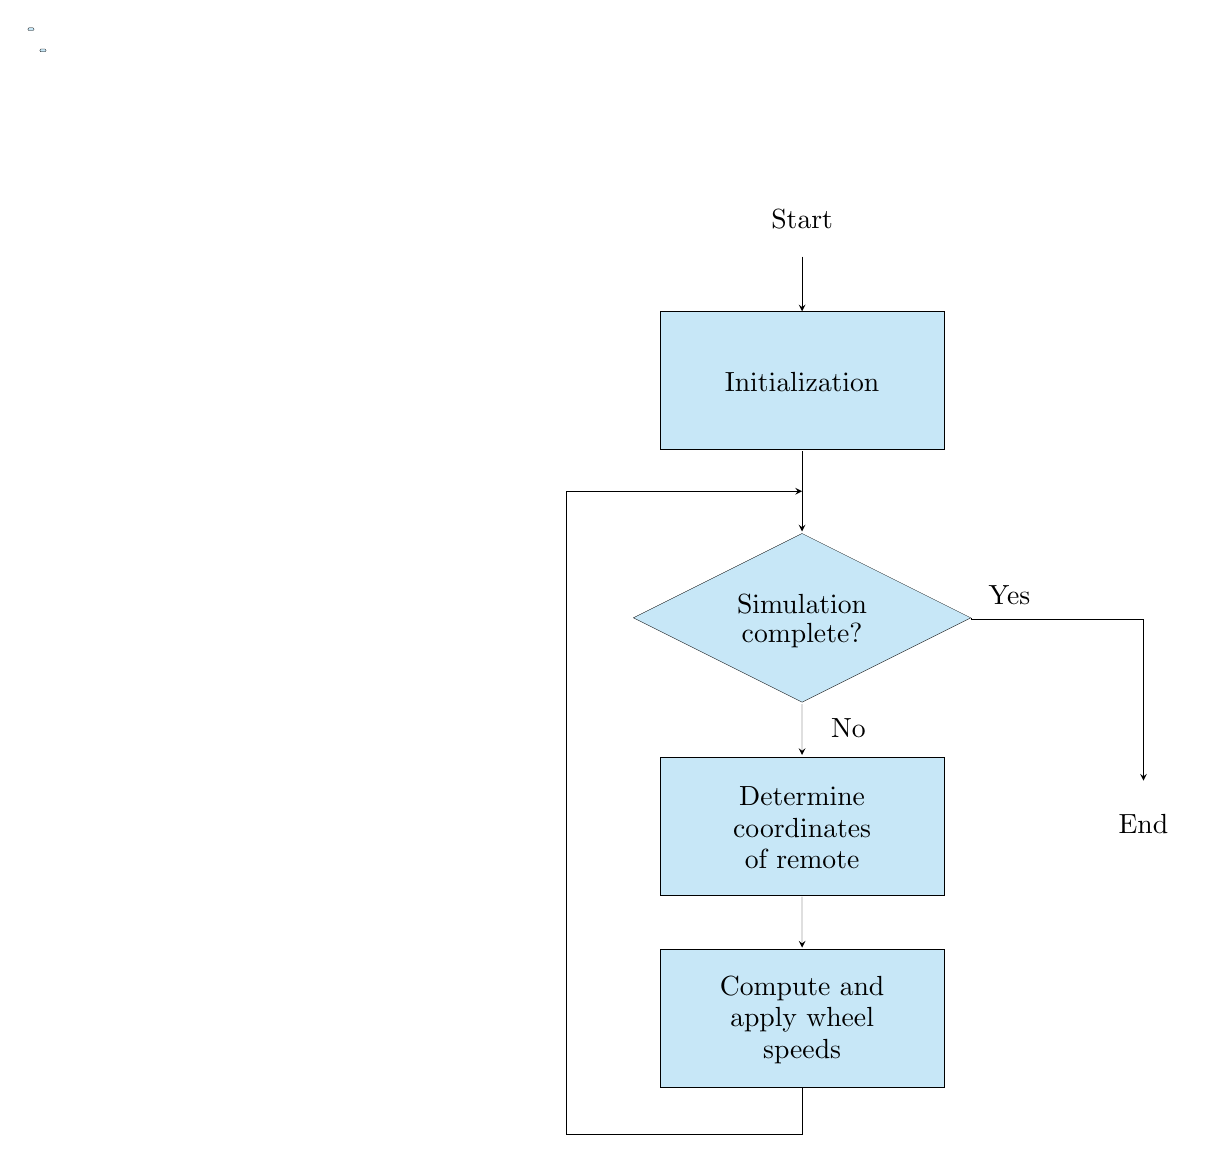
\begin{tikzpicture}[scale=0.5]
\pgftransformxscale{1.000000}
\pgftransformyscale{-1.000000}
\definecolor{dialinecolor}{rgb}{0.000000, 0.000000, 0.000000}
\pgfsetstrokecolor{dialinecolor}
\definecolor{dialinecolor}{rgb}{1.000000, 1.000000, 1.000000}
\pgfsetfillcolor{dialinecolor}
\pgfsetlinewidth{0.100000\du}
\pgfsetdash{}{0pt}
\pgfsetdash{}{0pt}
\pgfsetbuttcap
\pgfsetmiterjoin
\pgfsetlinewidth{0.100000\du}
\pgfsetbuttcap
\pgfsetmiterjoin
\pgfsetdash{}{0pt}
\definecolor{dialinecolor}{rgb}{0.780392, 0.905882, 0.968627}
\pgfsetfillcolor{dialinecolor}
\pgfpathmoveto{\pgfpoint{18.786863\du}{3.950000\du}}
\pgfpathlineto{\pgfpoint{21.813113\du}{3.950000\du}}
\pgfpathcurveto{\pgfpoint{22.230951\du}{3.950000\du}}{\pgfpoint{22.569675\du}{4.397715\du}}{\pgfpoint{22.569675\du}{4.950000\du}}
\pgfpathcurveto{\pgfpoint{22.569675\du}{5.502285\du}}{\pgfpoint{22.230951\du}{5.950000\du}}{\pgfpoint{21.813113\du}{5.950000\du}}
\pgfpathlineto{\pgfpoint{18.786863\du}{5.950000\du}}
\pgfpathcurveto{\pgfpoint{18.369024\du}{5.950000\du}}{\pgfpoint{18.030300\du}{5.502285\du}}{\pgfpoint{18.030300\du}{4.950000\du}}
\pgfpathcurveto{\pgfpoint{18.030300\du}{4.397715\du}}{\pgfpoint{18.369024\du}{3.950000\du}}{\pgfpoint{18.786863\du}{3.950000\du}}
\pgfusepath{fill}
\definecolor{dialinecolor}{rgb}{0.000000, 0.000000, 0.000000}
\pgfsetstrokecolor{dialinecolor}
\pgfpathmoveto{\pgfpoint{18.786863\du}{3.950000\du}}
\pgfpathlineto{\pgfpoint{21.813113\du}{3.950000\du}}
\pgfpathcurveto{\pgfpoint{22.230951\du}{3.950000\du}}{\pgfpoint{22.569675\du}{4.397715\du}}{\pgfpoint{22.569675\du}{4.950000\du}}
\pgfpathcurveto{\pgfpoint{22.569675\du}{5.502285\du}}{\pgfpoint{22.230951\du}{5.950000\du}}{\pgfpoint{21.813113\du}{5.950000\du}}
\pgfpathlineto{\pgfpoint{18.786863\du}{5.950000\du}}
\pgfpathcurveto{\pgfpoint{18.369024\du}{5.950000\du}}{\pgfpoint{18.030300\du}{5.502285\du}}{\pgfpoint{18.030300\du}{4.950000\du}}
\pgfpathcurveto{\pgfpoint{18.030300\du}{4.397715\du}}{\pgfpoint{18.369024\du}{3.950000\du}}{\pgfpoint{18.786863\du}{3.950000\du}}
\pgfusepath{stroke}
% setfont left to latex
\definecolor{dialinecolor}{rgb}{0.000000, 0.000000, 0.000000}
\pgfsetstrokecolor{dialinecolor}
\node at (20.299988\du,4.990000\du){Start};
\definecolor{dialinecolor}{rgb}{0.780392, 0.905882, 0.968627}
\pgfsetfillcolor{dialinecolor}
\fill (16.698800\du,18.658900\du)--(16.698800\du,22.158900\du)--(23.901300\du,22.158900\du)--(23.901300\du,18.658900\du)--cycle;
\pgfsetlinewidth{0.100000\du}
\pgfsetdash{}{0pt}
\pgfsetdash{}{0pt}
\pgfsetmiterjoin
\definecolor{dialinecolor}{rgb}{0.000000, 0.000000, 0.000000}
\pgfsetstrokecolor{dialinecolor}
\draw (16.698800\du,18.658900\du)--(16.698800\du,22.158900\du)--(23.901300\du,22.158900\du)--(23.901300\du,18.658900\du)--cycle;
% setfont left to latex
\definecolor{dialinecolor}{rgb}{0.000000, 0.000000, 0.000000}
\pgfsetstrokecolor{dialinecolor}
\node at (20.300050\du,19.648900\du){Determine};
% setfont left to latex
\definecolor{dialinecolor}{rgb}{0.000000, 0.000000, 0.000000}
\pgfsetstrokecolor{dialinecolor}
\node at (20.300050\du,20.448900\du){coordinates};
% setfont left to latex
\definecolor{dialinecolor}{rgb}{0.000000, 0.000000, 0.000000}
\pgfsetstrokecolor{dialinecolor}
\node at (20.300050\du,21.248900\du){of remote};
\definecolor{dialinecolor}{rgb}{0.780392, 0.905882, 0.968627}
\pgfsetfillcolor{dialinecolor}
\fill (16.698700\du,7.341080\du)--(16.698700\du,10.841080\du)--(23.901200\du,10.841080\du)--(23.901200\du,7.341080\du)--cycle;
\pgfsetlinewidth{0.100000\du}
\pgfsetdash{}{0pt}
\pgfsetdash{}{0pt}
\pgfsetmiterjoin
\definecolor{dialinecolor}{rgb}{0.000000, 0.000000, 0.000000}
\pgfsetstrokecolor{dialinecolor}
\draw (16.698700\du,7.341080\du)--(16.698700\du,10.841080\du)--(23.901200\du,10.841080\du)--(23.901200\du,7.341080\du)--cycle;
% setfont left to latex
\definecolor{dialinecolor}{rgb}{0.000000, 0.000000, 0.000000}
\pgfsetstrokecolor{dialinecolor}
\node at (20.299950\du,9.131080\du){Initialization};
\definecolor{dialinecolor}{rgb}{0.780392, 0.905882, 0.968627}
\pgfsetfillcolor{dialinecolor}
\fill (16.698700\du,23.550000\du)--(16.698700\du,27.050000\du)--(23.901200\du,27.050000\du)--(23.901200\du,23.550000\du)--cycle;
\pgfsetlinewidth{0.100000\du}
\pgfsetdash{}{0pt}
\pgfsetdash{}{0pt}
\pgfsetmiterjoin
\definecolor{dialinecolor}{rgb}{0.000000, 0.000000, 0.000000}
\pgfsetstrokecolor{dialinecolor}
\draw (16.698700\du,23.550000\du)--(16.698700\du,27.050000\du)--(23.901200\du,27.050000\du)--(23.901200\du,23.550000\du)--cycle;
% setfont left to latex
\definecolor{dialinecolor}{rgb}{0.000000, 0.000000, 0.000000}
\pgfsetstrokecolor{dialinecolor}
\node at (20.299950\du,24.540000\du){Compute and};
% setfont left to latex
\definecolor{dialinecolor}{rgb}{0.000000, 0.000000, 0.000000}
\pgfsetstrokecolor{dialinecolor}
\node at (20.299950\du,25.340000\du){apply wheel};
% setfont left to latex
\definecolor{dialinecolor}{rgb}{0.000000, 0.000000, 0.000000}
\pgfsetstrokecolor{dialinecolor}
\node at (20.299950\du,26.140000\du){speeds};
\definecolor{dialinecolor}{rgb}{0.780392, 0.905882, 0.968627}
\pgfsetfillcolor{dialinecolor}
\fill (20.299960\du,12.982200\du)--(24.585620\du,15.125030\du)--(20.299960\du,17.267860\du)--(16.014300\du,15.125030\du)--cycle;
\pgfsetlinewidth{0.100000\du}
\pgfsetdash{}{0pt}
\pgfsetdash{}{0pt}
\pgfsetmiterjoin
\definecolor{dialinecolor}{rgb}{0.000000, 0.000000, 0.000000}
\pgfsetstrokecolor{dialinecolor}
\draw (20.299960\du,12.982200\du)--(24.585620\du,15.125030\du)--(20.299960\du,17.267860\du)--(16.014300\du,15.125030\du)--cycle;
% setfont left to latex
\definecolor{dialinecolor}{rgb}{0.000000, 0.000000, 0.000000}
\pgfsetstrokecolor{dialinecolor}
\node at (20.299960\du,14.765030\du){Simulation};
% setfont left to latex
\definecolor{dialinecolor}{rgb}{0.000000, 0.000000, 0.000000}
\pgfsetstrokecolor{dialinecolor}
\node at (20.299960\du,15.565030\du){complete?};
\pgfsetlinewidth{0.100000\du}
\pgfsetdash{}{0pt}
\pgfsetdash{}{0pt}
\pgfsetbuttcap
\pgfsetmiterjoin
\pgfsetlinewidth{0.100000\du}
\pgfsetbuttcap
\pgfsetmiterjoin
\pgfsetdash{}{0pt}
\definecolor{dialinecolor}{rgb}{0.780392, 0.905882, 0.968627}
\pgfsetfillcolor{dialinecolor}
\pgfpathmoveto{\pgfpoint{27.457863\du}{19.310600\du}}
\pgfpathlineto{\pgfpoint{30.484113\du}{19.310600\du}}
\pgfpathcurveto{\pgfpoint{30.901951\du}{19.310600\du}}{\pgfpoint{31.240675\du}{19.758315\du}}{\pgfpoint{31.240675\du}{20.310600\du}}
\pgfpathcurveto{\pgfpoint{31.240675\du}{20.862885\du}}{\pgfpoint{30.901951\du}{21.310600\du}}{\pgfpoint{30.484113\du}{21.310600\du}}
\pgfpathlineto{\pgfpoint{27.457863\du}{21.310600\du}}
\pgfpathcurveto{\pgfpoint{27.040024\du}{21.310600\du}}{\pgfpoint{26.701300\du}{20.862885\du}}{\pgfpoint{26.701300\du}{20.310600\du}}
\pgfpathcurveto{\pgfpoint{26.701300\du}{19.758315\du}}{\pgfpoint{27.040024\du}{19.310600\du}}{\pgfpoint{27.457863\du}{19.310600\du}}
\pgfusepath{fill}
\definecolor{dialinecolor}{rgb}{0.000000, 0.000000, 0.000000}
\pgfsetstrokecolor{dialinecolor}
\pgfpathmoveto{\pgfpoint{27.457863\du}{19.310600\du}}
\pgfpathlineto{\pgfpoint{30.484113\du}{19.310600\du}}
\pgfpathcurveto{\pgfpoint{30.901951\du}{19.310600\du}}{\pgfpoint{31.240675\du}{19.758315\du}}{\pgfpoint{31.240675\du}{20.310600\du}}
\pgfpathcurveto{\pgfpoint{31.240675\du}{20.862885\du}}{\pgfpoint{30.901951\du}{21.310600\du}}{\pgfpoint{30.484113\du}{21.310600\du}}
\pgfpathlineto{\pgfpoint{27.457863\du}{21.310600\du}}
\pgfpathcurveto{\pgfpoint{27.040024\du}{21.310600\du}}{\pgfpoint{26.701300\du}{20.862885\du}}{\pgfpoint{26.701300\du}{20.310600\du}}
\pgfpathcurveto{\pgfpoint{26.701300\du}{19.758315\du}}{\pgfpoint{27.040024\du}{19.310600\du}}{\pgfpoint{27.457863\du}{19.310600\du}}
\pgfusepath{stroke}
% setfont left to latex
\definecolor{dialinecolor}{rgb}{0.000000, 0.000000, 0.000000}
\pgfsetstrokecolor{dialinecolor}
\node at (28.970988\du,20.350600\du){End};
\pgfsetlinewidth{0.100000\du}
\pgfsetdash{}{0pt}
\pgfsetdash{}{0pt}
\pgfsetbuttcap
{
\definecolor{dialinecolor}{rgb}{0.000000, 0.000000, 0.000000}
\pgfsetfillcolor{dialinecolor}
% was here!!!
\pgfsetarrowsend{stealth}
\definecolor{dialinecolor}{rgb}{0.000000, 0.000000, 0.000000}
\pgfsetstrokecolor{dialinecolor}
\draw (20.300000\du,5.950000\du)--(20.300000\du,7.341080\du);
}
\pgfsetlinewidth{0.100000\du}
\pgfsetdash{}{0pt}
\pgfsetdash{}{0pt}
\pgfsetbuttcap
{
\definecolor{dialinecolor}{rgb}{0.000000, 0.000000, 0.000000}
\pgfsetfillcolor{dialinecolor}
% was here!!!
\pgfsetarrowsend{stealth}
\definecolor{dialinecolor}{rgb}{0.000000, 0.000000, 0.000000}
\pgfsetstrokecolor{dialinecolor}
\draw (20.299953\du,10.889775\du)--(20.299956\du,12.932202\du);
}
\pgfsetlinewidth{0.100000\du}
\pgfsetdash{}{0pt}
\pgfsetdash{}{0pt}
\pgfsetbuttcap
{
\definecolor{dialinecolor}{rgb}{0.000000, 0.000000, 0.000000}
\pgfsetfillcolor{dialinecolor}
% was here!!!
\pgfsetarrowsend{stealth}
\definecolor{dialinecolor}{rgb}{0.000000, 0.000000, 0.000000}
\pgfsetstrokecolor{dialinecolor}
\draw (20.299997\du,17.317846\du)--(20.300019\du,18.610630\du);
}
\pgfsetlinewidth{0.100000\du}
\pgfsetdash{}{0pt}
\pgfsetdash{}{0pt}
\pgfsetbuttcap
{
\definecolor{dialinecolor}{rgb}{0.000000, 0.000000, 0.000000}
\pgfsetfillcolor{dialinecolor}
% was here!!!
\pgfsetarrowsend{stealth}
\definecolor{dialinecolor}{rgb}{0.000000, 0.000000, 0.000000}
\pgfsetstrokecolor{dialinecolor}
\draw (20.300013\du,22.207239\du)--(20.299987\du,23.501661\du);
}
\pgfsetlinewidth{0.100000\du}
\pgfsetdash{}{0pt}
\pgfsetdash{}{0pt}
\pgfsetmiterjoin
\pgfsetbuttcap
{
\definecolor{dialinecolor}{rgb}{0.000000, 0.000000, 0.000000}
\pgfsetfillcolor{dialinecolor}
% was here!!!
\pgfsetarrowsend{stealth}
{\pgfsetcornersarced{\pgfpoint{0.000000\du}{0.000000\du}}\definecolor{dialinecolor}{rgb}{0.000000, 0.000000, 0.000000}
\pgfsetstrokecolor{dialinecolor}
\draw (20.300000\du,27.050000\du)--(20.300000\du,28.250000\du)--(14.300000\du,28.250000\du)--(14.300000\du,11.911000\du)--(20.300000\du,11.911000\du);
}}
\pgfsetlinewidth{0.100000\du}
\pgfsetdash{}{0pt}
\pgfsetdash{}{0pt}
\pgfsetmiterjoin
\pgfsetbuttcap
{
\definecolor{dialinecolor}{rgb}{0.000000, 0.000000, 0.000000}
\pgfsetfillcolor{dialinecolor}
% was here!!!
\pgfsetarrowsend{stealth}
{\pgfsetcornersarced{\pgfpoint{0.000000\du}{0.000000\du}}\definecolor{dialinecolor}{rgb}{0.000000, 0.000000, 0.000000}
\pgfsetstrokecolor{dialinecolor}
\draw (24.585700\du,15.125000\du)--(24.585700\du,15.151500\du)--(28.970990\du,15.151500\du)--(28.970988\du,19.261398\du);
}}
% setfont left to latex
\definecolor{dialinecolor}{rgb}{0.000000, 0.000000, 0.000000}
\pgfsetstrokecolor{dialinecolor}
\node[anchor=west] at (24.800000\du,14.550000\du){Yes};
% setfont left to latex
\definecolor{dialinecolor}{rgb}{0.000000, 0.000000, 0.000000}
\pgfsetstrokecolor{dialinecolor}
\node[anchor=west] at (20.797500\du,17.925000\du){No};
\end{tikzpicture}

    \endgroup
    \caption{Flowchart of Navigation Algorithm}
    \label{fig:navAlgo}
  \end{figure}
\end{frame}

\begin{frame}{Navigation Algorithm}
  \centering
  \scalebox{0.8}{
  \begin{algorithm}[H]
    \SetAlgoLined
    \KwIn{Signal Strengths from Remote}
    \KwOut{Mobile Robot Trajectory}
    \Begin
    {
      Initialize sampling time $T > 0$, following distance $d_f$, $K_p$, $K_\omega$\\
      \While{true}
      {
        Estimate distance $d_{Ref}$ to remote using signal strength\\
        Estimate angle $\theta_{Ref}$ to remote using signal strengths\\
        Compute target point with respect to robot's local frame as $x_{Ref} = (d_{Ref} - d_f)\cos \theta_{Ref}$, $y_{Ref} = (d_{Ref} - d_f)\sin \theta_{Ref}$\\
        Compute linear speed $v(t) = sign(x_{Ref})K_p\sqrt{x_{Ref}^2 + y_{Ref}^2}$\\
        Compute $\omega(t) = K_\omega \theta_{Ref}$\\
        Compute left and right wheel speeds for robot\\
        Apply wheel speeds to robot\\
      }
    }
    \caption{Navigation Algorithm}
    \label{alg:navAlgo}
  \end{algorithm}}
\end{frame}

%----------------------------------

\section{Schedule}

\begin{frame}{Fall Semester Schedule}

    \begin{figure}
      \centering
      \begin{ganttchart}[
        hgrid,
        vgrid,
        x unit=.27cm,
        y unit title=.5cm,
        y unit chart=.27cm,
        title label font=\scriptsize,
        milestone label font=\tiny,
        milestone progress label font = \tiny,
        milestone progress label anchor = east,
        bar label font=\tiny,
        group label font=\footnotesize,
        bar/.append style={fill=green},
        bar incomplete/.append style={fill=red},
        group progress label font = \tiny,
        progress label text={$\displaystyle####1\%$},
        group progress label anchor = east,
        bar progress label font = \tiny,
        bar progress label anchor = east,
        ]{1}{17}

        \gantttitle{2020}{17}\\
        \gantttitle{Sep}{4}
        \gantttitle{Oct}{4}
        \gantttitle{Nov}{4}
        \gantttitle{Dec}{4}
        \gantttitle{}{1}\\
    
        \ganttgroup[progress = 100]{Research}{3}{12} \\
        \ganttbar[progress = 100]{Research Multipath}{3}{12}\\
        \ganttbar[progress = 100]{Research Reflector}{3}{12}\\

        \ganttgroup[progress = 80]{Simulation}{8}{10}\\
        \ganttbar[progress = 80]{CoppeliaSim simulation}{8}{10}\\
        \ganttmilestone[progress = 0]{Simulation Complete}{10}\\

        \ganttgroup[progress = 90]{Project Proposal}{11}{12}\\
        \ganttbar[progress = 90]{Proposal Document}{11}{11}\\
        \ganttbar[progress = 90]{Proposal Presentation}{12}{12}\\

        \ganttgroup[progress = 90]{XBee Setup}{13}{14}\\
        \ganttbar[progress = 90]{Voltage Regulator Circuit}{13}{13}\\
        \ganttbar[progress = 90]{Configuration with X-CTU}{14}{14}\\
        \ganttbar[progress = 90]{Sensing RSSI}{14}{14}\\
        \ganttbar[progress = 90]{UART Communication}{14}{14}\\
      \end{ganttchart}
    \caption{Gantt chart for Fall 2020}
    \label{fig:gantt1}
  \end{figure}
  
\end{frame}

%----------------------------------

\begin{frame}{Spring Semester Schedule}
\begin{figure}
  \centering
  \begin{ganttchart}[
    hgrid,
    vgrid,
    x unit=.25cm,
    y unit title=.45cm,
    y unit chart=.25cm,
    title label font=\scriptsize,
    milestone label font=\tiny,
    milestone progress label font = \tiny,
    milestone progress label anchor = east,
    bar label font=\tiny,
    group label font=\footnotesize,
    bar/.append style={fill=green},
    bar incomplete/.append style={fill=red},
    group progress label font = \tiny,
    progress label text={$\displaystyle####1\%$},
    group progress label anchor = east,
    bar progress label font = \tiny,
    bar progress label anchor = east,
    ]{1}{20}
    \gantttitle{2020}{20}\\
    \gantttitle{Jan}{3}
    \gantttitle{Feb}{4}
    \gantttitle{Mar}{4}
    \gantttitle{Apr}{4}
    \gantttitle{May}{4}
    \gantttitle{}{1}\\

    \ganttgroup[progress = 0]{Assembly}{3}{4}\\
    \ganttbar[progress = 0]{Replace Motors}{3}{3}\\
    \ganttbar[progress = 0]{Design and Construct Reflector}{3}{4}\\
    \ganttbar[progress = 0]{Mount Reflector}{4}{4}\\
    \ganttmilestone[progress = 0]{Assembly Complete}{4}\\

    \ganttgroup[progress = 40]{Software}{5}{6}\\
    \ganttbar[progress = 80]{XBee Library}{5}{5}\\
    \ganttbar[progress = 0]{Control Algorithm}{6}{6}\\

    \ganttgroup[progress = 0]{Angle Estimation}{7}{8}\\
    \ganttbar[progress = 0]{Rotate XBee on Stepper Motor}{7}{7}\\
    \ganttbar[progress = 0]{Determine Angle}{8}{8}\\

    \ganttgroup[progress = 0]{Distance Estimation}{9}{10}\\
    \ganttbar[progress = 0]{Calibrate Distance Calculation}{9}{10}\\

    \ganttgroup[progress = 0]{Subsystem Integration}{11}{15}\\
    \ganttbar[progress = 0]{Angle Estimation Testing}{11}{11}\\
    \ganttbar[progress = 0]{Distance Estimation Testing}{12}{13}\\
    \ganttbar[progress = 0]{System Testing}{14}{15}\\
    \ganttmilestone[progress = 0]{Integration Complete}{15}\\

    \ganttgroup[progress = 0]{Project Completion}{16}{17}\\
    \ganttbar[progress = 0]{Final Report}{16}{16}\\
    \ganttbar[progress = 0]{Final Presentation}{17}{17}\\
    \ganttbar[progress = 0]{Presentation to IAB}{17}{17}\\
    \ganttbar[progress = 0]{Project Demo}{17}{17}\\

    \ganttmilestone[progress = 0]{Project Complete}{17}
  \end{ganttchart}
  \caption{Gantt Chart for Spring 2020}
  \label{fig:gantt2}
\end{figure}
\end{frame}

%----------------------------------

\section{Anticipated Challenges}
\begin{frame}{Anticipated Challenges}
  \begin{block}{Challenges}
    \begin{itemize}
      \item Inaccurate distance measurements due to multipath effect from environment
      \item Achieving full 360\textdegree measurement in short enough time
    \end{itemize}
  \end{block}
\end{frame}

%----------------------------------

\section{Concluding Remarks}
\begin{frame}{}
  \begin{block}{Concluding Remarks}
    \begin{LARGE}
      \begin{itemize}
        \item Proposed robotic cart system uses analog RF signal strength to locate and follow the user
        \begin{itemize}
          \item Does not require line-of-sight
          \item Low-cost
        \end{itemize}
      \end{itemize}
    \end{LARGE}
  \end{block}
\end{frame}

%----------------------------------

\section{References}

% \begin{frame}{References}
%   \bibliographystyle{IEEEtran}
%   \begin{itemize}
%     \item N. Rawashdeh, R. Haddad, O. Jadallah, and A. To’ma, “A person-following
% robotic cart controlled via a smartphone application: design and evaluation,”
% 09 2017, pp. 1–5.
%     \item M. M. Islam, A. Lam, H. Fukuda, Y. Kobayashi, and Y. Kuno, “An intelligent
% shopping support robot: understanding shopping behavior from 2d skeleton data using gru network,” ROBOMECH Journal, vol. 6, no. 1, 2019.
%     \item J. Sales, J. Marti, R. Marin Prades, E. Cervera, and P. Sanz, “Comparob: The
% shopping cart assistance robot,” International Journal of Distributed Sensor Networks, vol. 2016, pp. 1–15, 02 2016.
%     \item M. S. Miah, J. Knoll, and K. Hevrdejs, “Intelligent range-only mapping and navigation for mobile robots,” IEEE Transactions on Industrial Informatics, vol. 14, no. 3, pp. 1164–1174, 2018.
%     \item D. Li and S. Lane, “A novel and versatile parabolic reflector that significantly
% improves wi-fi reception at different distances and angles,” 2013.
  
%   \end{itemize}


% \end{frame}

%----------------------------------

\begin{frame}{References}

  \bibliographystyle{IEEEtran}
  \bibliography{bib/references.bib}
% 	\begin{itemize}
% 		\item T. Xie, H. Jiang, X. Zhao, and C. Zhang, “A wi-fi-based wireless indoor position sensing system with multipath interference mitigation,” Sep 2019. [Online].
% Available: https://www.ncbi.nlm.nih.gov/pmc/articles/PMC6767237/
% 		\item A. M. Ladd, K. E. Bekris, A. Rudys, L. E. Kavraki, and D. S. Wallach, “Robotics-
% based location sensing using wireless ethernet,” Wireless Networks, vol. 11, no. 1-2, p. 189–204, 2005.
% 		\item M. Lindhe, K. Johansson, and A. Bicchi, “An experimental study of exploiting multipath fading for robot communications,” Robotics: Science and Systems III, 2007.
% 		\item M. Lindhe and K. Johansson, “Using robot mobility to exploit multipath fading,”Wireless Communications, IEEE, vol. 16, pp. 30 – 37, 03 2009.
% 	\end{itemize}

\end{frame}


\end{document}



%%% Local Variables:
%%% mode: latex
%%% TeX-master: t
%%% End:
